\documentclass[12pt]{exam}
\usepackage{amsthm}
\usepackage{libertine}
\usepackage[utf8]{inputenc}
\usepackage[margin=1in]{geometry}
\usepackage{amsmath,amssymb}
\usepackage{multicol}
\usepackage[shortlabels]{enumitem}
\usepackage{siunitx}
\usepackage{cancel}
\usepackage{graphicx}
\usepackage{pgfplots}
\usepackage{listings}
\usepackage{tikz}


\pgfplotsset{width=10cm,compat=1.9}
\usepgfplotslibrary{external}
\tikzexternalize

\newcommand{\class}{Moderna - Complementaria} % This is the name of the course 
\newcommand{\examnum}{Taller 5} % This is the name of the assignment
\newcommand{\examdate}{24/02/2023} % This is the due date
\newcommand{\timelimit}{}





\begin{document}
\pagestyle{plain}
\thispagestyle{empty}

\noindent
\begin{tabular*}{\textwidth}{l @{\extracolsep{\fill}} r @{\extracolsep{6pt}} l}
\textbf{\class} & \textbf{Name:} & \textit{David Pachon}\\ %Your name here instead, obviously 
	\textbf{\examnum} && \textit{Sergio Montoya}\\
\textbf{\examdate} &&\\
\end{tabular*}\\
\rule[2ex]{\textwidth}{2pt}
% ---

\begin{enumerate}
	\item Demuestre, usando la ley de Plank, que se puede evitar la catástrofe ultravioleta encontrando la intensidad cuando $\lambda \rightarrow 0$.
		Para esto, vamos a asumir un valor constante para la variable T dado que nos piden el valor solamente el valor cuando la longitud de onda tiende a 0. Por lo tanto, ademas de eso vamos a montar una simplificación de la ley de plaank que conserve las generalidades de los puntos.
		\begin{align*}
			& I(\lambda, T) = \frac{2\pi c^2h}{\lambda^5}\frac{1}{e^{\frac{hc}{\lambda K_B T}}}\Rightarrow I(\lambda)=\frac{1}{x^5}\frac{1}{e^{\frac{1}{x}}}\\
		\end{align*}
		Si hacemos un limite en ambas funciones por separado nos queda que
		\begin{align}
			& \lim_{x\to 0}\frac{1}{x} = \infty\\
			& \lim_{x\to 0}\frac{1}{e^{\frac{1}{x}}} = 0\\
		\end{align}
		Sin embargo, dado que (2) tiende a 0 "mas rapido", entonces el valor de la intensidad en este caso seria 0. Para ejemplificar esto se adjunta una grafica de ambas curvas
		\begin{figure}[h]
			\centering
			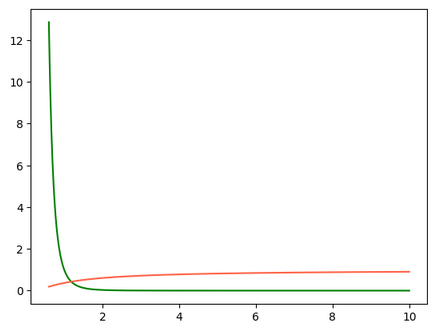
\includegraphics[scale=0.6]{Grafica1.png}
			\caption{Graficas de las funciones simplificadas de la leey de Plank}
		\end{figure}
	\item De la formula general nos quedamos con las siguientes dos ecuaciones
		\begin{align*}
			&V_1e=\frac{ch}{\lambda_1}-\phi\\
			&V_2e=\frac{ch}{\lambda_2}-\phi
		\end{align*}
		De esas dos lo que hacemos ahora es expresarlas en función de h lo que nos queda como 
		\begin{align*}
			&h = \frac{(V_2e-V_1e)(\lambda_1\lambda_2)}{(\lambda_1 - \lambda_2)c}
		\end{align*}
		Ahora reemplazamos con los valores dados y quedamos con resultado igual a
		\begin{align*}
			&h = 4.4\times 10^{-15}eV\cdot s
		\end{align*}
		Por ultimo, con esta información hallamos el valor de $\phi$ el cual es
		\begin{align*}
			&\phi = 4.07 eV
		\end{align*}
	\item Primero debemos desarrollar una expresión desde la información dada
		\begin{align*}
			& \frac{\Delta \lambda}{\lambda} = 0.004\\
			& \Delta \lambda = 0.004 \lambda\\
			& \text{Por la ecuación de Compton tenemos }\Delta \lambda\\
			& \frac{h}{m_e c}(1-\cos(\theta))=0.004\lambda\\
			& \frac{\frac{h}{m_e c}(1-\cos(\theta))}{0.004}=\lambda
		\end{align*}
		Ahora bien, si ponemos todos estos valores en una calculadora y reemplazamos para cada $\theta$ entonces nos queda
		\begin{enumerate}
			\item $\lambda = 4.42\times 10^{-5}$
			\item $\lambda = 0.00033$
			\item $\lambda = 0.00065$
		\end{enumerate}
\end{enumerate}



\end{document}
